%%%%%%%%%%%%%%%%%%%%%%%%%%%%%%%%%%%%%%%%%%%%%%%
%%% Template for lab reports used at STIMA
%%%%%%%%%%%%%%%%%%%%%%%%%%%%%%%%%%%%%%%%%%%%%%%

%%%%%%%%%%%%%%%%%%%%%%%%%%%%%% Sets the document class for the document Openany
% is added to remove the book style of starting every new chapter on an odd page
% (not needed for reports)
\documentclass[11pt,english, openright, oneside]{book}

%%%%%%%%%%%%%%%%%%%%%%%%%%%%%% Loading packages that alter the style
\usepackage[]{graphicx}
\usepackage[]{color}
\usepackage{alltt}
\usepackage[T1]{fontenc}
\usepackage[utf8]{inputenc}
\usepackage{subcaption}
\usepackage{listings}
\usepackage{afterpage}
\newcommand\blankpage{%
    \null
    \thispagestyle{empty}%
    \newpage}

\usepackage[english, portuguese]{babel}

\usepackage[colorlinks = true, linkcolor = blue, urlcolor  = blue, citecolor =
            blue, anchorcolor = blue]{hyperref}

\newcommand{\MYhref}[3][blue]{\href{#2}{\color{#1}{#3}}}%

\renewcommand{\lstlistingname}{Anexos de Código}
\renewcommand{\lstlistlistingname}{Lista de \lstlistingname}

\setcounter{secnumdepth}{3}
\setcounter{tocdepth}{3}
\setlength{\parskip}{\smallskipamount}
\setlength{\parindent}{0pt}

\usepackage{listings}
\usepackage{color}

\definecolor{dkgreen}{rgb}{0,0.6,0}
\definecolor{gray}{rgb}{0.5,0.5,0.5}
\definecolor{mauve}{rgb}{0.58,0,0.82}
% Define some colors - Do professor
\definecolor{ListingColorKeyWord}{rgb}{0, 0.5, 0}
\definecolor{ListingColorComment}{rgb}{0.0, 0.0, 0.6}
\definecolor{ListingColorIdentifier}{rgb}{0.5, 0.12, 0.10}
\definecolor{ListingColorEmphasize}{rgb}{0, 1, 1}

\definecolor{ListingColorBreakLine}{rgb}{0.5, 0.12, 0.10}

\lstset{frame=tb, language=Java, aboveskip=3mm, belowskip=3mm,
  showstringspaces=false, columns=flexible, basicstyle={\small\ttfamily},
  numbers=none, numberstyle=\tiny\color{gray}, keywordstyle=\color{blue},
  commentstyle=\color{dkgreen}, stringstyle=\color{mauve}, breaklines=true,
  breakatwhitespace=true, tabsize=3 }

\lstset{ language=Python, keywordstyle={\color{ListingColorKeyWord}\bfseries},
	commentstyle=\color{ListingColorComment},
	identifierstyle=\color{ListingColorIdentifier}, basicstyle=\ttfamily,
	frame=single, showstringspaces=false, numbers=left, tabsize=2,
	breaklines=true,
	postbreak=\mbox{\textcolor{ListingColorBreakLine}{$\hookrightarrow$}}, }


\lstdefinelanguage{HTML5}{ language=html, sensitive=true, alsoletter={<>=-},
        otherkeywords={
        % HTML tags
        <html>, <head>, <title>, </title>, <meta, />, </head>, <body>, <canvas,
        \/canvas>, <script>, </script>, </body>, </html>, <!, html>, <style>,
        </style>, >< },  
        ndkeywords={
        % General
        =,
        % HTML attributes
        charset=, id=, width=, height=,
        % CSS properties
        border:, transform:, -moz-transform:, transition-duration:,
        transition-property:, transition-timing-function: },  
        morecomment=[s]{<!--}{-->}, tag=[s] }

\lstdefinelanguage{JavaScript}{ morekeywords={typeof, new, true, false, catch,
  function, return, null, catch, switch, var, if, in, while, do, else, case,
  break}, morecomment=[s]{/*}{*/}, morecomment=[l]//, morestring=[b]",
  morestring=[b]' }

% Set page margins
\usepackage[top=100pt,bottom=100pt,left=68pt,right=66pt]{geometry}

% Package used for placeholder text
\usepackage{lipsum}

% Prevents LaTeX from filling out a page to the bottom
\raggedbottom

% Adding both languages \usepackage[english, italian, portuguese]{babel}



\lstset{ language=python, %% Troque para PHP, C, Java, etc... bash é o padrão
    basicstyle=\ttfamily\small, numberstyle=\footnotesize, numbers=left,
    frame=single, tabsize=2, rulecolor=\color{black!30}, title=\lstname,
    escapeinside={\%*}{*)}, breaklines=true, breakatwhitespace=true,
    framextopmargin=2pt, framexbottommargin=2pt, inputencoding=utf8,
    extendedchars=true, literate={á}{{\'a}}1 {ã}{{\~a}}1 {é}{{\'e}}1
    {ç}{{\c{c}}}1, }


% All page numbers positioned at the bottom of the page
\usepackage{fancyhdr}
\fancyhf{} % clear all header and footers
\fancyfoot[C]{\thepage}
\renewcommand{\headrulewidth}{0pt} % remove the header rule
\pagestyle{fancy}
\renewcommand{\headrulewidth}{0.4pt}

% Changes the style of chapter headings
\usepackage{titlesec}
\titleformat{\chapter}
   {\normalfont\LARGE\bfseries}{\thechapter.}{1em}{}
% Change distance between chapter header and text
\titlespacing{\chapter}{0pt}{5pt}{2\baselineskip}

% Adds table captions above the table per default
\usepackage{float}
\floatstyle{plaintop}
\restylefloat{table}

% Adds space between caption and table
\usepackage[tableposition=top]{caption}

% Adds hyperlinks to references and ToC
\usepackage{hyperref}
\hypersetup{hidelinks,linkcolor = black} % Changes the link color to black and
% hides the hideous red border that usually is created

% If multiple images are to be added, a folder (path) with all the images can be
% added here 
\graphicspath{ {Figures/} }

% Separates the first part of the report/thesis in Roman numerals
\frontmatter

\usepackage{listings}
\usepackage{color}

\usepackage{titlesec}
\titleformat{\chapter}[display]
  {\centering \normalsize \huge  \color{black}}{\thechapter}{10pt}{}



\definecolor{dkgreen}{rgb}{0,0.6,0}
\definecolor{gray}{rgb}{0.5,0.5,0.5}
\definecolor{mauve}{rgb}{0.58,0,0.82}

\lstset{frame=tb, language=Java, aboveskip=3mm, belowskip=3mm,
  showstringspaces=false, columns=flexible, basicstyle={\small\ttfamily},
  numbers=none, numberstyle=\tiny\color{gray}, keywordstyle=\color{blue},
  commentstyle=\color{dkgreen}, stringstyle=\color{mauve}, breaklines=true,
  breakatwhitespace=true, tabsize=3 }

%%%%%%%%%%%%%%%%%%%%%%%%%%%%%% Starts the document
\begin{document}

%%% Selects the language to be used for the first couple of pages
\selectlanguage{portuguese}


\renewcommand{\contentsname}{Índice}

%%%%% Adds the title page
\begin{titlepage}
	\clearpage\thispagestyle{empty}
	\centering
	\vspace{1cm}

	% Titles Information about the University
	{\Large \textbf{Redes de Internet}\par} {\Large Departamento de Engenharia
	Eletrónica e Telecomunicações e de Computadores \par} {\Large Instituto
	Superior de Engenharia de Lisboa \par}
		
	\vspace{0.5cm}
    
    \centering 
\includegraphics[scale=0.7]{imagens/isel.png}

	\vspace{1cm}
	
	{\Huge \textbf{Trabalho nº 1 (VLAN/STP/RIP)}} \\
	\vspace{1cm}

        {\Large Licenciatura em Engenharia Informática e Multimédia}
        
	\vspace{1cm}
	
	
	
	
	\begin{center}
	{\normalsize Docente: \par Prof. Nuno Cruz \\
	
        \vspace{0.5cm}
              
        Alunos (Grupo 05):
        \par
        Alexandre Ferreira nº47485 
        \par 
        João Gonçalves nº47507
        \par
        Filipe Mendes nº48628
        
        \vspace{0.5cm} 
        Turma 52D
                
        \vspace{1cm}
        {\normalsize \today \par}
	             
	             
	             
	             \par}
	\end{center}
		
	% Set the date
	
	
	\pagebreak

\end{titlepage}

\tableofcontents
% Adds a table of contents
\pagebreak
\newpage


% Adds list of figures
\begingroup
\let\clearpage\relax
\pagebreak
\listoffigures
\endgroup

\newpage

% Adds list of tables
\begingroup
\let\clearpage\relax
\pagebreak
\listoftables
\endgroup

\newpage

\mainmatter
\chapter{Introdução}
Este relatório científico, elaborado no âmbito da disciplina de Redes de
Internet (RI), tem como objetivo aprofundar os conhecimentos sobre VLANs,
protocolos STP e RSTP, encaminhamento estático e RIP. O trabalho foi
desenvolvido em grupo, utilizando o simulador Packet Tracer, e envolveu a
criação e configuração de uma topologia de rede que representa uma
infraestrutura simplificada de um Internet Service Provider (ISP) e duas
empresas clientes.

\vspace{0.4cm}

Ao longo do trabalho, foram implementadas diversas tarefas que incluíram a
configuração de VLANs, a aplicação de protocolos de encaminhamento e a simulação
de cenários de redundância e falhas. O relatório detalha as configurações
realizadas, as justificações das escolhas efetuadas e os resultados obtidos,
proporcionando uma visão abrangente das técnicas e práticas utilizadas na gestão
e operação de redes de computadores.

\chapter{Desenvolvimento}

\section{Tarefa 1}
\vspace{0.2cm}

Implementar a rede correspondente à Empresa A e responder às questões
apresentadas (não se esqueça de justificar as suas respostas):  

\vspace{0.8cm}

\textbf{a) Use o comando: "no ip domain-lookup". Qual o objetivo deste comando?}
\vspace{0.2cm}

O comando \textbf{"no ip domain-lookup"} é utilizado para desativar a pesquisa
de DNS num router. Vai evitar atrasos quando se cometem erros de digitação ou
comandos inválidos, pois vai desativar o router de tentar resolver nomes no
domínio desconhecidos.
\vspace{0.8cm}


\textbf{b) Quais as VLAN por omissão que existem [sh vlan] antes de ser configurada qualquer VLAN em qualquer equipamento?}
\vspace{0.2cm}

Existem 5 \textit{VLANs}: Default, fddi-default, token-ring-default,
fddinet-default, trnet-default.

Como se pode ver na figura \ref{fig:1b}
\vspace{0.4cm}

\begin{figure}[htp]
    \centering
    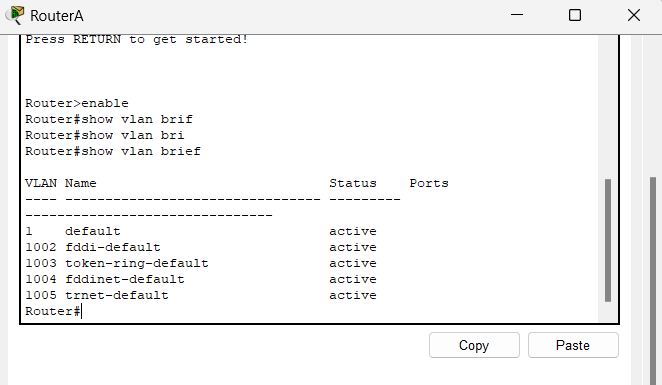
\includegraphics[width=0.6\textwidth]{imagens/Tarefa1/1.b.png}
    \caption{Tarefa 1 b) - VLANs no router A}
    \label{fig:1b}
\end{figure}

\vspace{0.8cm}


\pagebreak
\textbf{c) Qual o formato da tags introduzidas nas tramas Ethernet nas ligações trunk?}
\vspace{0.2cm}

Uma \textit{trunk} transporta várias \textit{VLANs} e, normalmente, são usadas
para ligações entre \textit{switches}. As tramas usadas nestas ligações contêm
campos adicionais para identificar a que VLAN pertencem.

O formato das tags segue o padrão \textit{\textbf{802.1Q}}, como se pode ver na
figura \ref{fig:1c}.
\vspace{0.4cm}

\begin{figure}[htp]
    \centering
    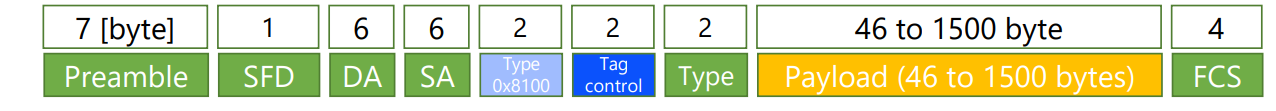
\includegraphics[width=0.8\textwidth]{imagens/Tarefa1/1.c.png}
    \caption{Tarefa 1 c) - Formato das tags 802.1Q}
    \label{fig:1c}
\end{figure} 

\vspace{0.8cm}


\textbf{d) Qual a razão pela qual, numa LAN que utilize VLANs, numa ligação tipo Access as tramas não incluem tags?}
\vspace{0.2cm}

Enquanto que uma porta trunk é usada em switches para transportar múltiplas
VLANs, a porta access é usada para conectar dispositivos finais à rede, como
PCs. Estes dispositivos não processam as tags da VLAN, por isso, não precisam se
preocupar com a segmentação em VLANs, pois a separação das ligações é uma
responsabilidade dos switches.
\vspace{0.8cm}


\textbf{e) Qual é a tag que as tramas pertencentes à VLAN 1 transportam?}
\vspace{0.2cm}

Por padrão, a VLAN nativa é VLAN 1 e, por isso, as tramas pertencentes a esta
VLAN são enviadas sem tag (untagged). Isto significa que quando uma interface
está configurada na VLAN 1, as tramas circulam nessa interface sem identificação
específica de VLAN. 

Se um dispositivo não suportar trunking, a circulação de tramas é possível
através da sua VLAN nativa.
\vspace{0.8cm}


\textbf{f) Uma máquina quando recebe uma trama Ethernet como diferencia se esta a seguir ao campo endereço de origem inclui o campo do tipo Type/Lenght ou se inclui os campos associados a uma VLAN?}
\vspace{0.2cm}

A máquina identifica a presença de uma tag VLAN verificando se o campo logo após
o endereço de origem é 0x8100. Se for, é uma trama com VLAN e, se não for, é uma
trama não está etiquetada com VLAN.
\vspace{0.8cm}


\pagebreak
\textbf{g) Quais as possíveis consequências de passarmos os timers “Max Age”=20 sec e “Forward Delay”= 15 sec para metade desses valores?}
\vspace{0.2cm}

Ao passarmos os timers "Max Age" e "Forward Delay" para metade dos seus valores
padrão podemos, por um lado, ser afetados positivamente na medida em que essa
mudança possibilita convergência mais rápida, podendo a rede ajustar-se mais
rapidamente a mudanças na topologia, como a adição ou remoção de dispositivos.
No entanto, as consequências negativas acabam por ser maiores pois adiciona-se
um maior risco de instabilidade e uma diminuição na resiliência a falha
temporárias. Passa a ser possível uma mais rápida mudança de estados e mudanças
como alterações na topologia, o que pode levar a que apareçam erros que não
existiriam, ou que seriam rapidamente solucionados, caso a rede convergisse com
menos rapidez.
\vspace{0.8cm}


\textbf{i) Qual é a Root Bridge (RB)? Justifique.}
\label{quest:1i}
\vspace{0.2cm}

O router SW\_DW é a root bridge porque a saída do switch diz "This bridge is the
root" e o endereço MAC no campo Address é o mesmo do SW\_DW.

Como se pode ver na figura \ref{fig:1i}
\vspace{0.4cm}
\begin{figure}[h]
    \centering
    \begin{subfigure}{.47\textwidth}
        \centering
        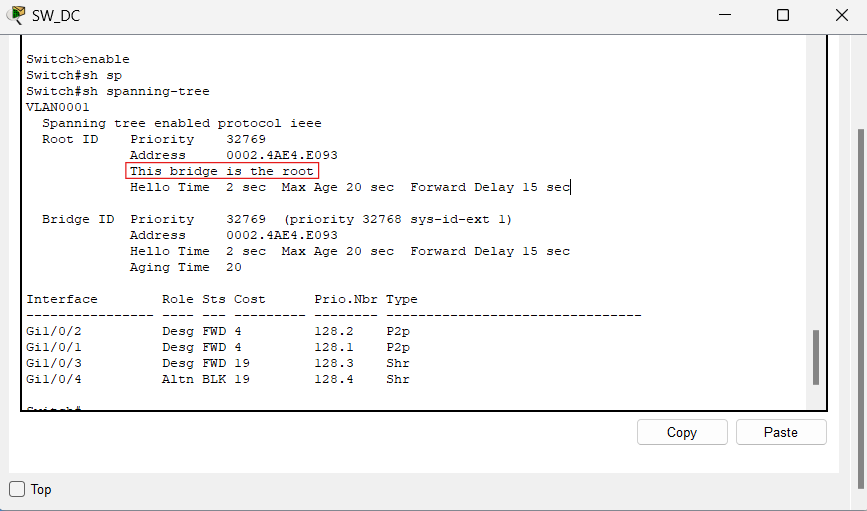
\includegraphics[width=0.99\linewidth]{imagens/Tarefa1/1.i.png}
    \end{subfigure}%
    \begin{subfigure}{.53\textwidth}
        \centering
        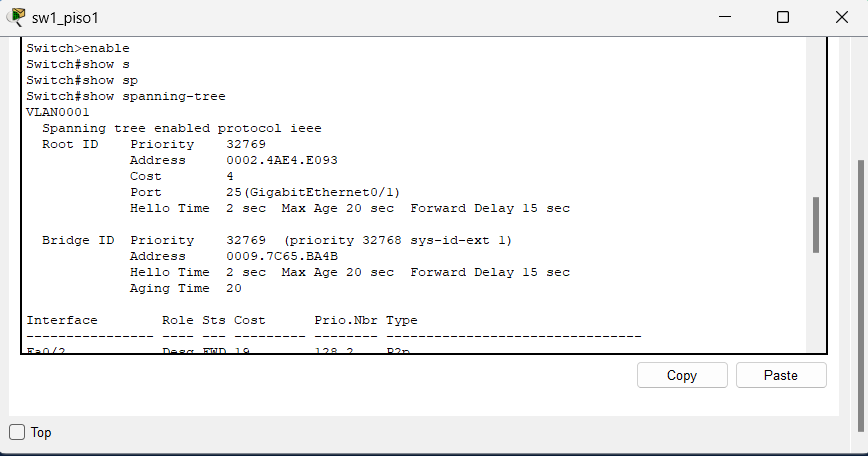
\includegraphics[width=0.99\linewidth]{imagens/Tarefa1/1.i.2.png}
    \end{subfigure}
    \caption{Tarefa 1 i) - Root Bridge}
    \label{fig:1i}
\end{figure}

\newpage

\textbf{j) Por omissão qual é o tipo de Spanning-Tree (STP) ativo [sh span]?}
\vspace{0.2cm}

Por omissão, o protocolo Spanning Tree Protocol em switches é o \textbf{IEEE
802.1D}.

Como se pode ver na figura \ref{fig:1j}
\vspace{0.4cm}

\begin{figure}[H]
    \centering
    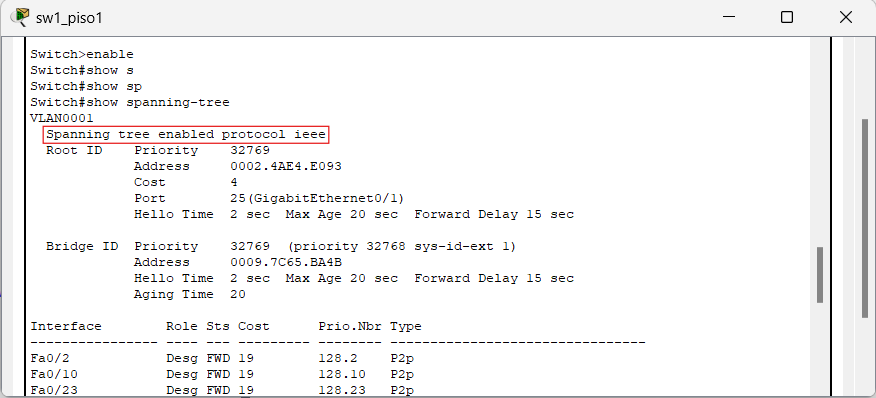
\includegraphics[width=0.6\textwidth]{imagens/Tarefa1/1.j.png}
    \caption{Tarefa 1 j) - comando sh span}
    \label{fig:1j}
\end{figure}

\vspace{0.8cm}

\textbf{k) Quantas árvores (spanning trees) existem na topologia implementada?}
\vspace{0.2cm}

Como usa o protocolo IEEE 802.1D, contêm apenas uma árvore que é criada para
cada VLAN. Ou seja, como só existe uma VLAN, só há uma árvore.

Como se pode ver na figura \ref{fig:1k}
\vspace{0.4cm}

\begin{figure}[H]
    \centering
    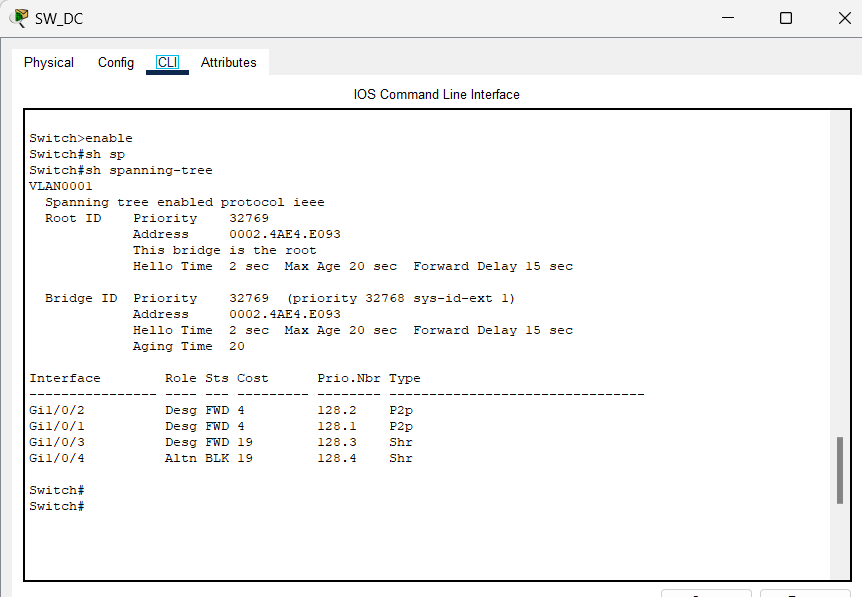
\includegraphics[width=0.6\textwidth]{imagens/Tarefa1/1.k.png}
    \caption{Tarefa 1 k) - Árvores}
    \label{fig:1k}
\end{figure}

\vspace{0.8cm}


\textbf{l) Para a empresa A, construa a tabela de cálculo do custo dos caminhos e de determinação de quais são as portas Root, Designated e Blocking e calcule os respetivos valores (verifique no PT quais os valores dos custos utilizados nos cálculos das spanning trees). Os resultados finais a que chegou são coerentes com os que o simulador PT apresenta?}
\vspace{0.2cm}

\begin{table}[h!]
\centering
\begin{tabular}{|c|c|c|c|c|c|c|}
 \hline
 \textbf{Porta} & \textbf{PC} & \textbf{RPC} & \textbf{RP} &  \textbf{DPC} &
 \textbf{DP} & \textbf{Block}\\
 \hline
 SW\_DC  Gi1/0/1 & 4 & - & - & 0 & X & -\\
 SW\_DC  Gi1/0/2 & 4 & - & - & 0 & X & -\\
 \hline
 \hline
 SW1\_P1  Fa0/2 & 19 & 23 & - & 4 & X & -\\
 SW1\_P1  Fa0/23 & 19 & 42 & - & 4 & X & -\\
 SW1\_P1  Fa0/24 & 18 & 41 & - & 4 & X & -\\
 SW1\_P1  Gi0/1 & 4 & 4 & X & - & - & -\\
 \hline
 \hline
 SW2\_P1  Fa0/1 & 19 & 60 & - & 4 & X & -\\
 SW2\_P1 Fa0/2 & 19 & 23 & - & 4 & - & X\\
 SW2\_P1  Gi0/1 & 4 & 4 & X & - & - & -\\
 SW2\_P1  Fa0/24 & 19 & 60 & - & 4 & X & -\\
 SW2\_P1  Fa0/23 & 19 & 41 & - & 4 & X & -\\
 \hline
 \hline
 SW1\_P2  Fa0/2 & 19 & 42 & - & 23 & - & X\\
 SW1\_P2  Fa0/18 & 19 & 23 & - & 22 & - & X\\
 SW1\_P2  Fa0/23 & 19 & 23 & - & 23 & - & X\\
 SW1\_P2  Fa0/24 & 19 & 22 & X & - & - & -\\
 \hline
 \hline
 SW2\_P2  Fa0/2 & 19 & 41 & - & 23 & X & -\\
 SW2\_P2  Fa0/1 & 19 & 23 & X & - & - & -\\
 SW2\_P2  Fa0/24 & 19 & 23 & - & 4 & - & X\\
 \hline
\end{tabular}
\caption{Spanning Tree}
\label{tab:span}
\end{table}
\vspace{0.8cm}


\textbf{m) Qual o custo do caminho mais curto até ao Router A desde o PC9?}
\vspace{0.2cm}

 O Custo do caminho mais curto do PC9 até ao Router A é 46.
 \vspace{0.1cm}
 
 \par PC9 -> SW2 Piso 2 = 19 \par SW2 Piso 2-> SW2 Piso 1 = 19 \par SW2 Piso 1->
 SW DC = 4 \par SW DC-> Router = 4
\vspace{0.8cm}


\textbf{n) Force a root bridge para ser o SW\_DC através da prioridade. Possui alguma porta bloqueada?}
\vspace{0.2cm}

Como foi respondido anteriormente na alínea i, SW\_DC é a root bridge.
\vspace{0.8cm}


\textbf{o) Na literatura sobre spanning tree encontra-se frequentemente a afirmação de que todas as portas de um root switch/bridge são portas Designated. Comente tendo em consideração o SW\_DC.}
\vspace{0.2cm}

Esta afirmação está correta de acordo com o funcionamento do STP. Sendo a root
bridge o ponto central da rede, todas as suas portas serão designated ports,
pois vão encaminhar tramas para outros switches sem bloqueios e loops.

Sendo SW\_DC a root bridge, todas as suas portas vão ser designated ports. No
entanto, na sua configuração tem duas portas a ligar ao mesmo dispositivo, por
isso, uma delas vai ser bloqueada para evitar possíveis loops.
\vspace{0.8cm}


\textbf{p) Ative o modo Per-Vlan Rapid Spanning Tree. Verifique se é necessário ativá-lo em todos os switches? }
\vspace{0.2cm}

Foi usado o comando "spanning-tree mode rapid-pvst" para mudar de protocolo no
switch. Apenas esse switch mudou, os outros continuam com o mesmo protocolo, por
isso, é preciso ativar em todos os switches.

Como se pode ver na figura \ref{fig:1p}
\vspace{0.4cm}
\begin{figure}[h]
    \centering
    \begin{subfigure}{.53\textwidth}
        \centering
        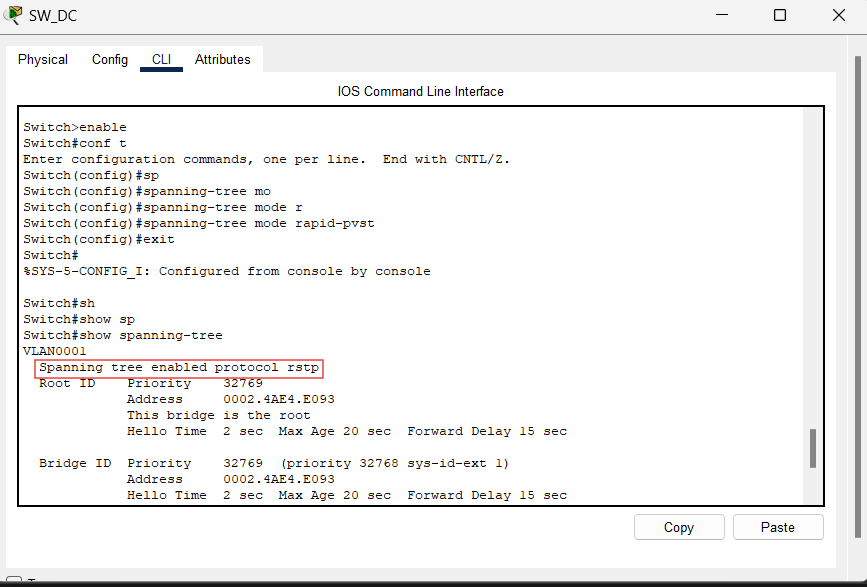
\includegraphics[width=0.99\linewidth]{imagens/Tarefa1/1.p.png}
    \end{subfigure}%
    \begin{subfigure}{.53\textwidth}
        \centering
        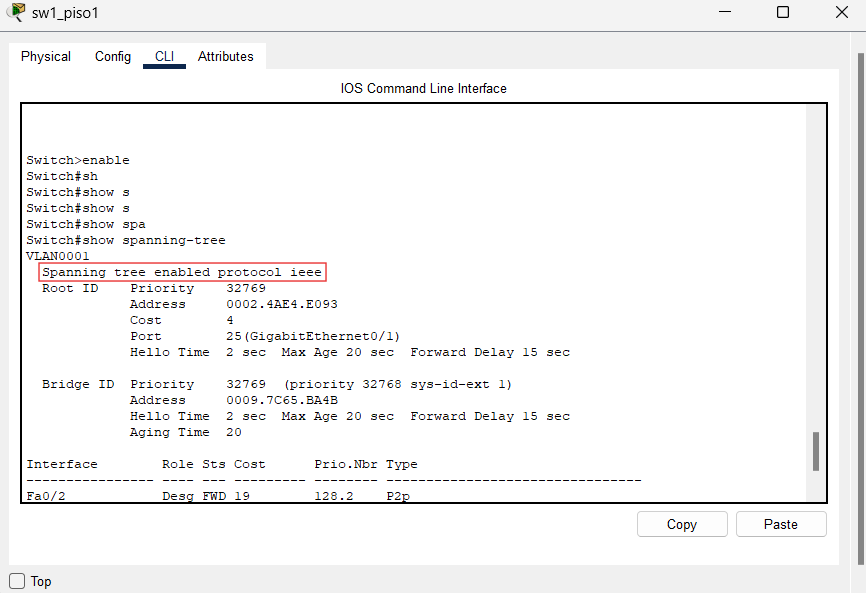
\includegraphics[width=0.99\linewidth]{imagens/Tarefa1/1.p.2.png}
    \end{subfigure}
    \caption{Tarefa 1 p) - Spanning Tree PVRST}
    \label{fig:1p}
\end{figure}
\vspace{0.8cm}


\textbf{q) Quantas árvores passaram a existir?}
\vspace{0.2cm}

Assim como no STP padrão, PVRST cria uma única árvore de spanning para cada
VLAN. Portanto, o número de árvores é o mesmo que o número de VLANs.
\vspace{0.8cm}

\newpage
\textbf{r) Existem duas ligações entre o sw1\_piso1 e o sw1\_piso2, uma delas bloqueada. Altere a configuração de maneira a desbloquear a ligação bloqueada e a desbloquear outra. [Opcional] Indique qual a forma de proceder de maneira que as duas ligações pudessem ser usadas em simultâneo.}
\vspace{0.2cm}

 As duas portas tem valores de custos diferentes, uma tem custo de 18 e a outra
 19. Para que seja possível a troca de estados, temos que aumentar o custo da
 porta de menor custo ou diminuir o da porta de maior custo. Para isso, usamos o
 comando "spanning-tree cost 100".
 
\vspace{0.8cm}


\textbf{s) Explique de forma detalhada a razão do sw2\_piso2 escolher o caminho por omissão em detrimento de outro possível. Realize as alterações que considerar necessárias para que o caminho preferido seja outro que não o escolhido (por omissão).}
\vspace{0.2cm}

Em cada switch será eleita uma porta Root Port, sendo esta aquela que consegue
garantir um menor custo de caminho até à Root Bridge. Entre as portas do Switch
2 do Piso 2, verifica-se que o caminho das duas interfaces (fa0/24 e fa0/1) até
à root bridge tem o mesmo custo de 23. Com isto, a porta mais pequena é
escolhida, sendo a outra bloqueada. 

Tal como aconteceu na anterior alínea, uma forma de alterar este caminho passa
por alterar o valor de custo de uma das portas. Se reduzirmos, essa é a
escolhida e se aumentarmos fica a outra. 
\vspace{0.8cm}


\textbf{t) Considere a seguinte afirmação: “Com o SW\_DC como root bridge, a substituição do Hub0 por um switch, interligado entre o sw1\_piso1 e o SW\_DC, iria melhor a conetividade entre o PC5 e o Server2 pois o caminho ficava mais curto.”. Indique, justificando, se a mesma é falsa ou verdadeira atendendo a que todas as ligações ao switch novo funcionam a 100 Mbps.}
\vspace{0.2cm}
 
Anteriormente, o PC5 passava pelo sw1\_piso1, SW\_DC, Hub0 até chegar ao
Server2. Com a subsituição do Hub0 por um switch e, fazendo a ligação com a root
bridge e sw1\_piso1 iremos ter um loop. Com isto, como as ligação do novo switch
tem um custo alto, as portas vão ser bloqueadas e, por isso, esta afirmação é
falsa, porque vai efetuar o mesmo percurso que fazia.
\vspace{0.8cm}

\pagebreak



\section{Tarefa 2}

Segmente a topologia da \textbf{Empresa A} utilizando VLAN para ficar de acordo
com as regras abaixo (poderá criar outras VLAN se necessário). Os informáticos
da empresa decidiram que cada VLAN terá um endereço IPv4 privado dentro da gama
\textbf{172.16.0.0/12}. A tabela seguinte é uma sugestão. Como resultado
pretende-se a implementação no  simulador da topologia indicada e o resultado
dos testes indicados na última alínea que comprovem que a topologia está
implementada e configurada como indicado nos passos (alíneas) seguintes:  

\begin{table}[h!]
\centering
\begin{tabular}{|c|c|c|c|c|}
\hline
\textbf{Nº Vlan} & \textbf{Nome} & \textbf{IP do Gateway} & \textbf{Rede} &  \textbf{PCs}\\
\hline
51 & Contabilidade & 172.24.51.254 & 172.24.51.0/24 & PC7, PC9\\
52 & Secretariado & 172.24.53.254 & 172.24.53.0/24 & PC5, PC8\\
53 & Informática & 172.24.55.126 & 172.24.55.0/25 & PC6\\
54 & Gestão da rede & 172.24.56.254 & 172.24.56.128/25 & Server2\\
\hline
\end{tabular}
\caption{VLANs da Empresa A}
\label{tab:vlansA}
\end{table}
\vspace{0.8cm}

\textbf{a) Configure as VLAN preferencialmente de acordo com a tabela anterior.}
\vspace{0.2cm}

Primeiramente, verificou-se em todos os switches a existência de VLANs, como se pode ver na figura \ref{fig:2a1}. 

\begin{figure}[H]
    \centering
    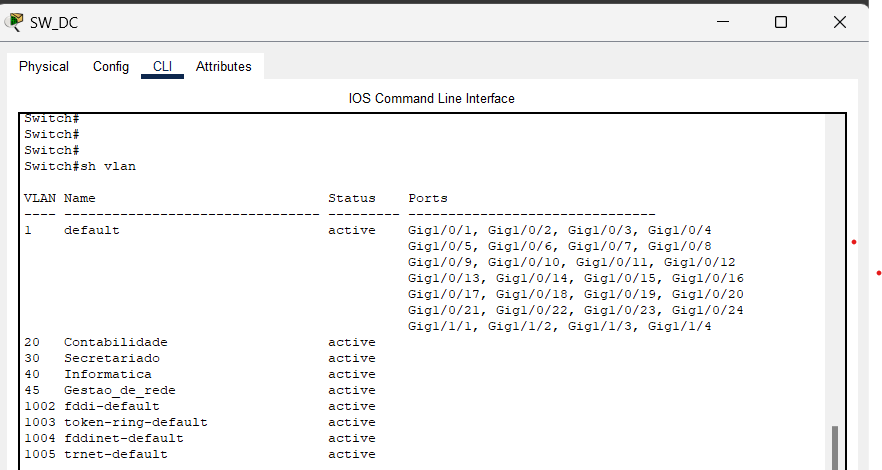
\includegraphics[width=0.6\textwidth]{imagens/Tarefa2/2.a.1.png}
    \caption{Tarefa 2 a) - Verificar VLANs}
    \label{fig:2a1}
\end{figure}

\vspace{0.2cm}

Caso existissem, eram eliminadas, como se pode ver na figura \ref{fig:2a2}.

\begin{figure}[H]
    \centering
    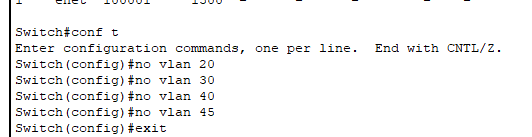
\includegraphics[width=0.6\textwidth]{imagens/Tarefa2/2.a.2.png}
    \caption{Tarefa 2 a) - Eliminar VLANs}
    \label{fig:2a2}
\end{figure}

\vspace{0.2cm}

De seguida, criaram-se as VLANs de acordo com a tabela fornecida, como se pode ver na figura \ref{fig:2a3}.

\begin{figure}[H]
    \centering
    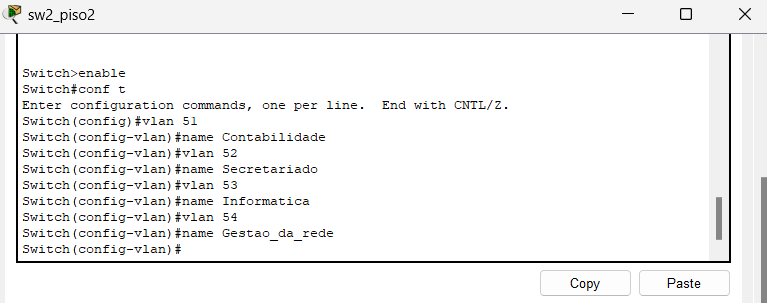
\includegraphics[width=0.6\textwidth]{imagens/Tarefa2/2.a.3.png}
    \caption{Tarefa 2 a) - Criar VLANs}
    \label{fig:2a3}
\end{figure}


A implementação de uma VLAN passa pelo uso do comando vlan (tag vlan) seguido de vlan (nome vlan). Assim sendo, executam-se, em cada switch, estes dois comandos para cada umas das 4 VLANs a implementar.

\vspace{0.8cm}

\textbf{b) Configure as portas em modo \textit{access} ou \textit{trunk} dependendo das necessidades. Desligue o protocolo \textit{Dynamic Trunking Protocol} (DTP) em cada interface que configurar como \textit{access} ou \textit{trunk}.}
\vspace{0.2cm}

Antes de começar a configurar as portas, é importante diferenciar os dois modos:

\begin{itemize}
    \item \textbf{Access:} é usado para conectar dispositivos finais à rede, como PCs. Estes dispositivos não processam as tags da VLAN, por isso, não precisam se preocupar com a segmentação em VLANs, pois a separação das ligações é uma responsabilidade dos switches.
    \item \textbf{Trunk:} é usado para transportar várias VLANs e, normalmente, são usadas para ligações entre switches. As tramas usadas nestas ligações contêm campos adicionais para identificar a que VLAN pertencem.
\end{itemize}

Com isto em mente, configuraram-se as portas de acordo com as necessidades de cada VLAN, como se pode ver na figura \ref{fig:2b}.
O Dynamic Trunking Protocol (DTP) é um protocolo que permite a negociação automática de troncos entre dois switches. No entanto, para evitar problemas de segurança, desativou-se o DTP usando o comando \textit{switchport nonegotiate}.

\begin{figure}[H]
    \centering
    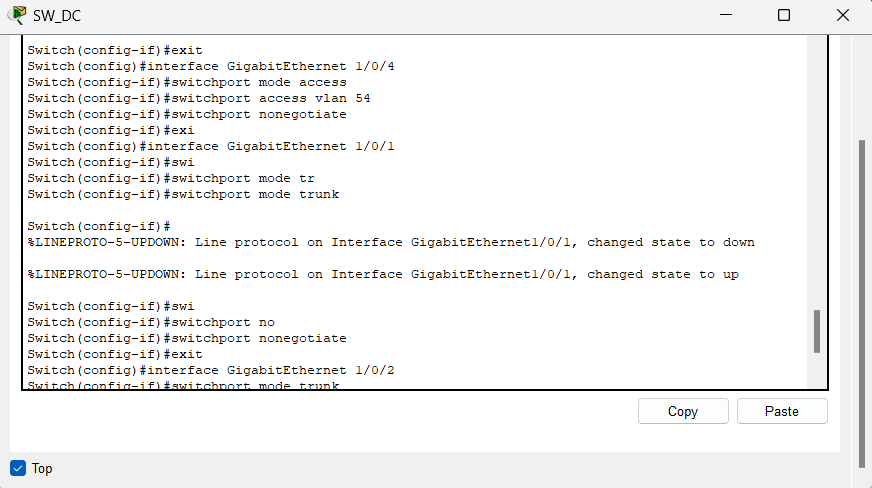
\includegraphics[width=0.6\textwidth]{imagens/Tarefa2/2.b.png}
    \caption{Tarefa 2 b) - Configurar portas}
    \label{fig:2b}
\end{figure}

\vspace{0.8cm}

\textbf{c) Configure o endereçamento IPv4 de todos os equipamentos tendo em consideração o sugerido na tabela. }
\vspace{0.2cm}

De acordo com a tabela das VLANs \ref{tab:vlansA}, configuraram-se os endereços IPV4 dos equipamentos, como se pode ver na tabela \ref{tab:ipA}.
\vspace{0.2cm}

\begin{table}[h!]
\centering
\begin{tabular}{|c|c|c|c|}
\hline
\textbf{Nº Vlan} & \textbf{Dispositivo} & \textbf{IPV4} & \textbf{IP do Gateway}\\
\hline
51 & PC7 & 172.24.51.1/24 & 172.24.51.254\\
51 & PC9 & 172.24.51.2/24 & 172.24.51.254\\
52 & PC5 & 172.24.53.1/24 & 172.24.53.254\\
52 & PC8 & 172.24.53.2/24 & 172.24.53.254\\
53 & PC6 & 172.24.55.1/25 & 172.24.55.126\\
54 & Server2 & 172.24.56.129/25 & 172.24.56.254\\
\hline
\end{tabular}
\caption{IPV4 Empresa A}
\label{tab:ipA}
\end{table}
\vspace{0.2cm}

Posteriormente, configuraram-se os endereços IPV4 dos equipamentos, como se pode ver na figura \ref{fig:2c}.
\vspace{0.2cm}

\begin{figure}[H]
    \centering
    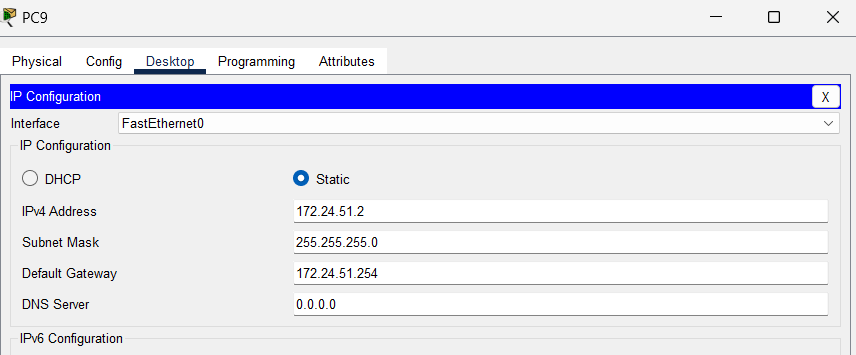
\includegraphics[width=0.6\textwidth]{imagens/Tarefa2/2.c.png}
    \caption{Tarefa 2 c) - Configurar IPV4}
    \label{fig:2c}
\end{figure}
    
\vspace{0.8cm}

\textbf{d) Verifique se existe conetividade entre os equipamentos em cada uma das VLAN.}
\vspace{0.2cm}

Para verificar a conectividade entre os equipamentos de cada VLAN, foi feito um teste de ping entre os dispositivos. O ping é uma ferramenta que permite testar a conectividade entre dois dispositivos numa rede, em que envia pacotes de dados para um dispositivo e espera por uma resposta. Este sinal é enviado através do protocolo ICMP (Internet Control Message Protocol) e é medido em milissegundos (ms).
Para testar, o PC9 vai fazer ping ao PC7 e os resultados foram positivos, como se pode ver na figura \ref{fig:2d}.

\begin{figure}[H]
    \centering
    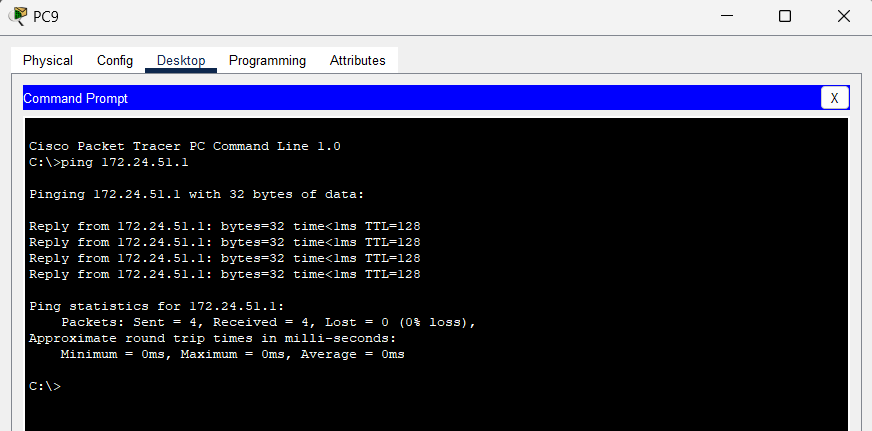
\includegraphics[width=0.6\textwidth]{imagens/Tarefa2/2.d.png}
    \caption{Tarefa 2 d) - Verificar conetividade}
    \label{fig:2d}
\end{figure}

\vspace{0.8cm}

\textbf{e) Verifique se existe conetividade entre os equipamentos de VLAN distintas.}
\vspace{0.2cm}

Para verificar a conectividade entre os equipamentos de VLAN distintas, foi feito um teste de ping entre os dispositivos. Para testar, o PC9 vai dar ping ao PC6 e, como não existe conectividade entre VLANs distintas, o ping não foi bem sucedido como se pode ver na figura \ref{fig:2e}.
Para que haja conectividade entre VLANs distintas, é necessário um router ou um switch layer 3. Assim, quando um dispositivo de uma VLAN quer comunicar com um dispositivo de outra VLAN, terá de um usar um endereço IP de gateway que permita a comunicação entre as VLANs. Desta forma, o tráfego passa pelo router ou switch layer 3 que faz a interligação entre as VLANs.

\begin{figure}[H]
    \centering
    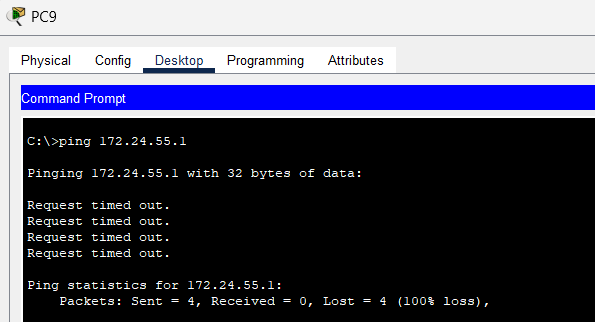
\includegraphics[width=0.6\textwidth]{imagens/Tarefa2/2.e.png}
    \caption{Tarefa 2 e) - Verificar conetividade}
    \label{fig:2e}
\end{figure}

\vspace{0.8cm}

\textbf{f) Ambas as ligações entre o hub Hub0 e o switch  SW\_DC estão ativas e deixam passar tráfego IPv4? Justifique.}
\vspace{0.2cm}

Ambas as ligações entre o hub Hub0 e o switch SW\_DC estão ativas e deixam passar tráfego IPv4. Isto acontece porque um hub é um dispositivo da camada 1 que opera na camada física do modelo OSI, ou seja, é um dispositivo que apenas replica o sinal que recebe para todas as portas. Assim, todas as portas do hub estão sempre ativas e, por isso, o tráfego IPv4 passa sem problemas. Já o switch SW\_DC é um dispositivo da camada 2 que opera na camada de ligação de dados do modelo OSI, ou seja, é um dispositivo que encaminha tramas para o destino correto. Assim, o tráfego IPv4 passa sem problemas.

\vspace{0.8cm}

\pagebreak


\section{Tarefa 3}
Ative o \textbf{RouterA} na topologia, ligando-o ao SW\_DC apenas configurando o RouterA e SW\_DC, segundo uma topologia \textit{router-on-a-stick}, e de acordo com as indicações que se seguem de maneira a estes ficarem com as configurações de acordo com as \textit{best practices}. Procure implementar, ao configurar as VLAN e o encaminhamento nos routers, as seguintes regras (sem recorrer a listas de acesso (ACL)) (Lembra-se que: Se no exterior de uma rede esta não for “conhecida”, os outros routers não enviarão tráfego para ela):

\textbf{Nota}: No futuro, quando evoluir na matéria de Redes, utilizando listas de acesso (ACL) irá constatar que podem ser implementadas com facilidade outras alternativas à limitação da comunicação (filtros) entre equipamentos em redes distintas, mas isso não é requerido neste trabalho dado que essa matéria será aprofundada apenas mais à frente

\underline{Lembre-se que cada rede/VLAN tem atribuídos endereços IPv4 públicos (apenas para uso nos routers)}
\underline{e privados. Do exterior das empresas só podem ser acedidos com endereços IPv4 públicos.}

\vspace{0.8cm}

\textbf{a) Configurar e ativar as \textit{interfaces} utilizadas de acordo com a regras enunciadas e as VLAN criadas (tenha em atenção que no uso de \textit{subinterfaces}, neste caso a correspondente interface física não possui configuração de IP).}
\vspace{0.2cm}

Começa-se por dividr a interface do router A em 4 subinterfaces, uma por VLAN, atribuindo a cada um o IP da default gateway da VLAN Associada.
Fazemos o comando \textit{no shutdown} para ativar a interface. Como se pode ver na figura \ref{fig:3a}.
\vspace{0.2cm}

\begin{figure}[H]
    \centering
    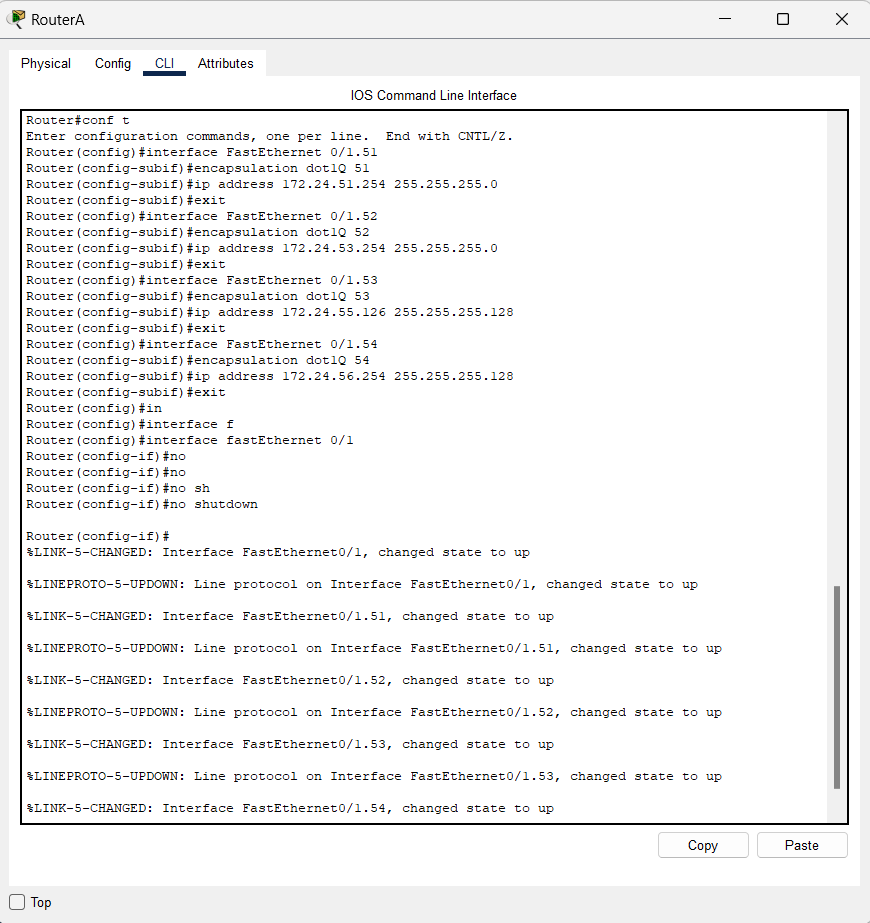
\includegraphics[width=0.6\textwidth]{imagens/Tarefa3/3.a.png}
    \caption{Tarefa 3 a) - Configurar interfaces}
    \label{fig:3a}
\end{figure}

\vspace{0.8cm}

\textbf{b) Atribuir o nome aos routers/switches com o comando hostname.}
\vspace{0.2cm}

Para atribuir um nome ao router, usamos o comando \textit{hostname} seguido do nome que queremos atribuir. Como se pode ver nas figuras \ref{fig:3b.1} e \ref{fig:3b.2}.
\vspace{0.2cm}

\begin{figure}[H]
    \centering
    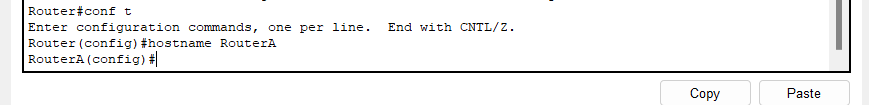
\includegraphics[width=0.6\textwidth]{imagens/Tarefa3/3.b.1.png}
    \caption{Tarefa 3 b) - Configurar nome RouterA}
    \label{fig:3b.1}
\end{figure}

\begin{figure}[H]
    \centering
    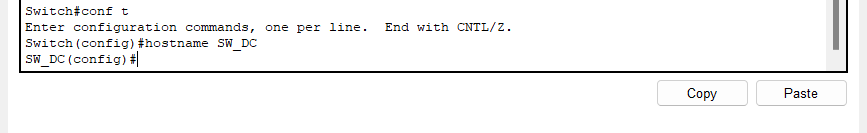
\includegraphics[width=0.6\textwidth]{imagens/Tarefa3/3.b.2.png}
    \caption{Tarefa 3 b) - Configurar nome SW\_DC}
    \label{fig:3b.2}
\end{figure}

\vspace{0.8cm}

\textbf{c) Configure uma mensagem inicial para quem entra no equipamento.}
\vspace{0.2cm}

Para configurar uma mensagem inicial, usamos o comando \textit{banner motd} seguido da mensagem que queremos que apareça. Como se pode ver na figura \ref{fig:3c}.
\vspace{0.2cm}

\begin{figure}[H]
    \centering
    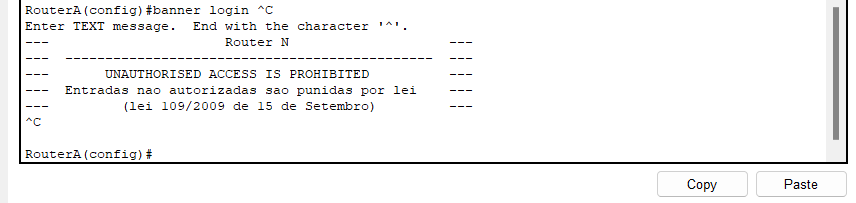
\includegraphics[width=0.6\textwidth]{imagens/Tarefa3/3.c.png}
    \caption{Tarefa 3 c) - Configurar mensagem inicial}
    \label{fig:3c}
\end{figure}

\vspace{0.8cm}

\textbf{d)	Salve as configurações no router não se esquecendo da primeira vez de verificar se ficou mesmo salvo, se funcionou.}
\vspace{0.2cm}

Para salvar as configurações, usamos o comando \textit{write memory} ou \textit{copy running-config startup-config}. Como se pode ver na figura \ref{fig:3d}.
\vspace{0.2cm}

\begin{figure}[H]
    \centering
    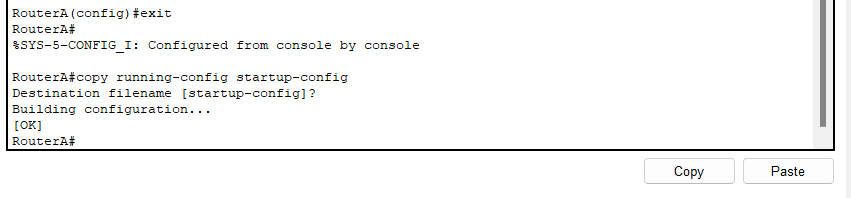
\includegraphics[width=0.6\textwidth]{imagens/Tarefa3/3.d.png}
    \caption{Tarefa 3 d) - Salvar configurações}
    \label{fig:3d}
\end{figure}

\vspace{0.8cm}

\textbf{e) Verifique se a conetividade entre os PC de diferentes VLAN. Pode utilizar o \textit{Ping}. Caso tenha problemas, faça o \textit{troubleshooting} para verificar se o problema está na \textit{vlan/rede} (possível causa nos \textit{switches/vlan} não criadas/passadas; portas em \textit{access/trunks} ou a própria configuração dos PC/endereçamento/máscara do PC/GW)) execute um \textit{ping} ao seu GW ou utilize um \textit{traceroute} para verificar em que “hop” está o problema. Se estiver a tentar “pingar” o PC7 do PC5 e se cada PC possuir conetividade com o seu GW, então o problema estará no \textit{router}.}
\vspace{0.2cm}

Para verificar a conectividade entre os PCs de diferentes VLAN, foi feito um teste de ping entre os dispositivos. Para testar, o PC7 vai dar ping ao Server2 e os resultados foram positivos, como se pode ver na figura \ref{fig:3.e.1}. Também podemos visualizar a tabela de arp do router A, onde podemos ver os endereços MAC associados a cada IP, como se pode ver na figura \ref{fig:3.e.2}.
\vspace{0.2cm}

\begin{figure}[H]
    \centering
    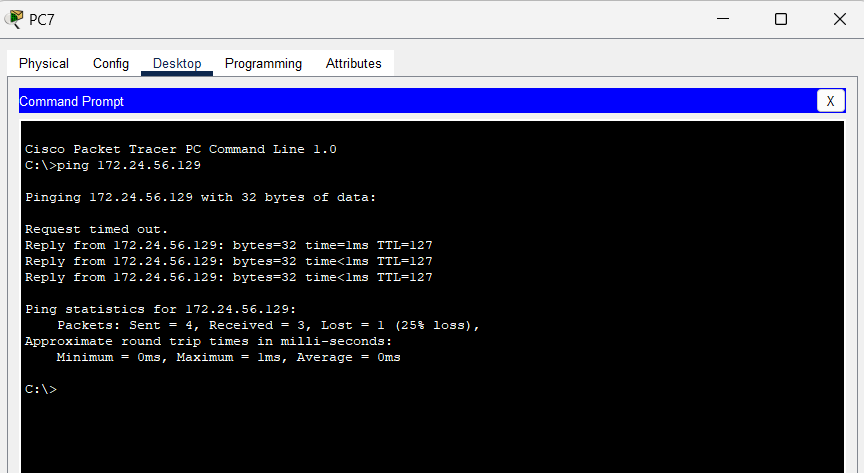
\includegraphics[width=0.6\textwidth]{imagens/Tarefa3/3.e.1.png}
    \caption{Tarefa 3 e) - Verificar conetividade}
    \label{fig:3.e.1}
\end{figure}

\begin{figure}[H]
    \centering
    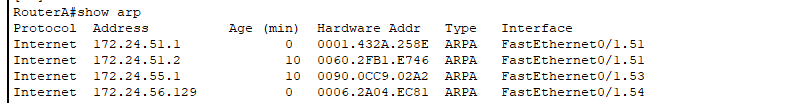
\includegraphics[width=0.6\textwidth]{imagens/Tarefa3/3.e.2.png}
    \caption{Tarefa 3 e) - Tabela ARP}
    \label{fig:3.e.2}
\end{figure}
\vspace{0.8cm}

\pagebreak

\section{Tarefa 4}
Implemente a topologia da \textbf{Empresa B}, sabendo que o ISP forneceu a esta duas redes blocos de endereços IPv4 públicos, mas que para efeitos de racionamento de endereçamento a Empresa B utiliza internamente blocos IPv4 privados /26, onde N representa o número do grupo.  
\vspace{0.2cm}

\begin{table}[h!]
    \centering
    \begin{tabular}{|c|c|c|c|c|}
    \hline
         \textbf{NºVlan} & \textbf{Nome} & \textbf{IP do Gateway} & \textbf{Rede} & \textbf{PCs}\\
    \hline
        2 & Servidores & 192.168.52.62 & 192.168.52.0/26 & Server1\\
        3 & Engenharia & 192.168.53.62 & 192.168.53.0/26 & PC1, PC2\\
    \hline
    \end{tabular}
    \caption{VLANs da Empresa B}
    \label{tab:vlansB}
\end{table}
\vspace{0.2cm}

De acordo com a tabela das VLANs \ref{tab:vlansB}, configuraram-se os endereços IPV4 dos equipamentos, como se pode ver na tabela \ref{tab:ipB}.
\vspace{0.2cm}

\begin{table}[h!]
    \centering
    \begin{tabular}{|c|c|c|c|}
    \hline
        \textbf{NºVlan} & \textbf{Dispositivos} & \textbf{IPV4} & \textbf{IP do Gateway}\\
    \hline
        2 & Server1 & 192.168.52.1/26 & 192.168.52.62\\
        3 & PC1 & 192.168.53.1/26 & 192.168.53.62\\
        3 & PC2 & 192.168.53.2/26 & 192.168.53.62\\
    \hline
    \end{tabular}
    \caption{IPV4 Empresa B}
    \label{tab:ipB}
\end{table}

\vspace{0.8cm}

\textbf{a) Será uma boa decisão, e era necessário, os informáticos da empresa B optarem por endereços IPv4 privados usando máscaras /26? Justifique.}
\vspace{0.2cm}

A escolha da Empresa B em utilizar endereços IPv4 privados com máscara /26 para suas VLANs é uma decisão acertada. Os endereços IPv4 públicos são limitados, e a adoção de endereços privados permite a criação de redes locais sem a necessidade de endereços públicos.

A máscara /26 possibilita a criação de quatro sub-redes, cada uma com até 62 endereços disponíveis, o que é suficiente para a quantidade de dispositivos presentes em cada VLAN. Além disso, o uso de endereços IPv4 privados é uma prática comum em redes locais, pois facilita a segmentação da rede e permite que os endereços públicos sejam utilizados apenas nos dispositivos que necessitam de comunicação com a Internet.

Portanto, a utilização de endereços IPv4 privados com máscara /26 é uma estratégia adequada e necessária para a Empresa B.

\pagebreak

\section{Tarefa 5}
Implemente a topologia do \textbf{ISP} de interligação com os clientes (empresas A e B e muitas outras não presentes na topologia):   
\vspace{0.8cm}

\textbf{a) Decida se nos routers do ISP é preferível utilizar endereços IPv4 privados ou públicos. Justifique.}
\vspace{0.2cm}

Nos routers do ISP, é preferível utilizar endereços IPv4 públicos. Esses endereços são únicos e globais, permitindo a comunicação com dispositivos em qualquer parte do mundo. Além disso, os endereços IPv4 públicos são essenciais para a conectividade com a Internet, uma vez que os endereços IPv4 privados não são roteáveis fora de uma rede local.

Para garantir a conectividade com os clientes e outros dispositivos na Internet, é imprescindível utilizar endereços IPv4 públicos nos roteadores do ISP. Essa prática assegura que todos os dados trafeguem de forma eficaz e que a comunicação entre diferentes redes seja mantida de maneira confiável.
\vspace{0.8cm}

\textbf{b) Relembre-se que quer o ISP quer as empresas possuem endereços IPv4 públicos e que as \underline{empresas só devem comunicar entre elas através dos \textit{routers} do ISP}. No caso de falha de um dos \textit{routers} do ISP, os \textit{routers} das empresas devem poder comunicar para fora através do outro \textit{router} do ISP (\textit{routers} 1 e 3).}

\textbf{Existe a possibilidade do ISP utilizar duas redes /30 (P2P em layer3) de interligação entre os seus routers e o de cada empresa.}

\textbf{As redes e respetivas VLAN podem ser: }
\begin{itemize}
    \item \textbf{VLAN 90 (EmpresaA) -> 10.5.90.0/30 }
    \item \textbf{VLAN 95 (EmpresaB) -> 10.5.95.4/30 }
\end{itemize}

\textbf{Se concluir que deve usar endereços IPv4 públicos nos equipamentos do ISP determine como pretende utilizar o bloco do ISP.}

\textbf{Atribua o endereçamento IP ao Router1, Router3, RouterA e RouterB, fazendo com que os routers do lado do ISP possuam sempre os primeiros endereços IP disponíveis na respetiva rede.}
\vspace{0.2cm}

\vspace{0.8cm}

\textbf{c) Configure os caminhos das VLAN na malha de \textit{switches} do ISP (configurando as interfaces em \textit{trunk} ou \textit{access} quando necessário), sabendo que para efeitos de redundância de camada 2, o ISP construiu um circuito entre as duas empresas, logo este é para ser usado apenas em caso necessário se os routers do ISP falharem. No caso de falha de um equipamento de rede deve ser possível manter o serviço mesmo que haja troços que fiquem com tráfego maior.}
\vspace{0.2cm}

\vspace{0.8cm}

\textbf{d) Verifique se existe conetividade ponto a ponto entre os \textit{routers} R1, RA, R3 e RB. Justifique.}
\vspace{0.2cm}

\vspace{0.8cm}


\chapter{Conclusões}



\chapter{Bibliografia}



\mainmatter



\afterpage{\blankpage}

\end{document}